% Made up for the tikra benchmark.
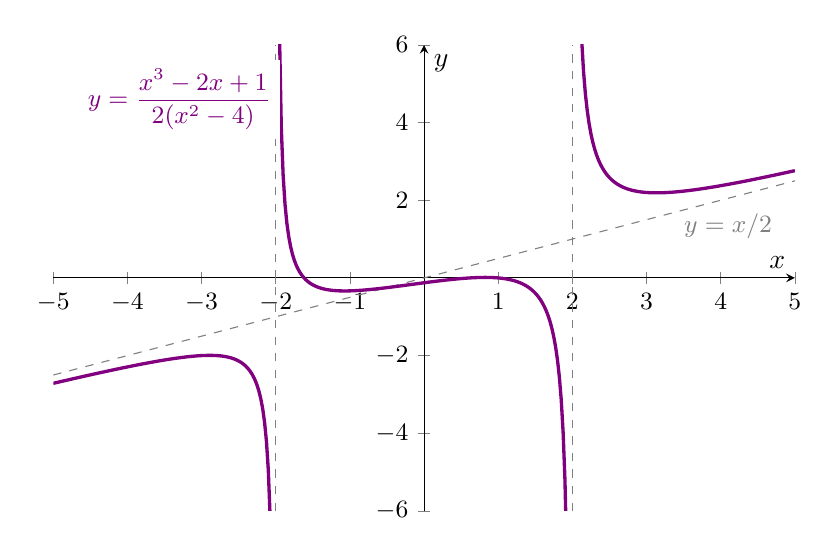
\begin{tikzpicture}
\begin{axis}[width=11cm, height=7.5cm, axis lines=middle, xmin=-5, xmax=5, ymin=-6, ymax=6,
    restrict y to domain=-12:12, unbounded coords=jump, samples=401, domain=-5:5,
    xlabel=$x$, ylabel=$y$, ticklabel style={font=\small}]
  \addplot[dashed, gray] coordinates {(-2,-6) (-2,6)};
  \addplot[dashed, gray] coordinates {(2,-6) (2,6)};
  \addplot[dashed, gray, domain=-5:5] {x/2};
  \addplot[very thick, violet] {(x^3 - 2*x + 1)/(2*(x^2 - 4))};
  \node[violet, fill=white, font=\small] at (axis cs:-3.3,4.6) {$\displaystyle y = \frac{x^3-2x+1}{2(x^2-4)}$};
  \node[gray, font=\small, anchor=north] at (axis cs:4.1,1.9) {$y = x/2$};
\end{axis}
\end{tikzpicture}
